\chapter{函数插值和重构}
\label{chap:interpolation}

\paragraph{基本问题}
已知关于某函数$f$的一组信息,如何重构$f$?事实上,由于信息缺失,无法准确重构。

\begin{definition}
    {重构}{}
    若$\{\phi_\alpha\}_{\alpha\in I}$是函数空间$X$上的一组线性无关泛函,给定某$f\in X$且$\phi_\alpha(f)$已知,希望确定$f^*\in Y\subset X$满足:
    \begin{equation}
        \phi_\alpha(f^*)=\phi_\alpha(f),\quad\forall\alpha\in I.
    \end{equation}
    $Y$称为插值空间或重构空间,$\{\phi_\alpha\}_{\alpha\in I}$为信息泛函。
\end{definition}

% \begin{remark}
%     几个基本问题:
%     \begin{itemize}
%         \item 存在性和唯一性;
%         \item 算法;
%         \item 合理性。
%     \end{itemize}
% \end{remark}

\begin{example}
    {采样空间的选择}{}
    \begin{itemize}
        \item 多项式函数空间
        \[
            \poly_n=\{a_0+a_1x+\cdots+a_nx^n\},
        \]
        \item 样条函数空间
        \item 三角多项式函数空间
        \[
            \mathcal Y_n=\{a_0+a_1\cos x+b_1\sin x+\cdots+a_n\cos nx+b_n\sin nx\}.
        \]
    \end{itemize}
\end{example}

\section{一维多项式插值}
\label{sec:1-D polynomial interpolation}

\subsection{Lagrange插值}

\begin{definition}
    {Lagrange插值}{Lagrange interpolation}
    插值空间$Y$由$n+1$个参数$a_0,\ldots,a_n$标定,即
    \[
        y=y(x;a_0,\ldots,a_n).
    \]
    给定一组插值节点(采样点) $x_i$和采样值$f_i=f(x_i)$,希望确定参数满足
    \begin{equation}
        y(x_i)=f(x_i),\quad\forall i\in I.
    \end{equation}
\end{definition}

\begin{theorem}
    {多项式插值定理}{}
    给定$n+1$个插值点$x_0,\ldots,x_n$,存在唯一的多项式函数$P_n\in\poly_n$满足插值条件。
\end{theorem}
\begin{proof}
    采取直接构造的方法。
    定义插值基函数
    \begin{equation}
        \ell_i(x):=\prod_{j\neq i}\frac{x-x_j}{x_i-x_j}.
    \end{equation}
    满足:
    \begin{equation}
        \ell_i(x_j)=\delta_{ij}.
    \end{equation}
    则插值多项式为
    \begin{equation}
        P_n(x)=\sum_{i=0}^nf(x_i)\ell_i(x).
        \qedhere
    \end{equation}
\end{proof}

\begin{definition}
    {余项}{}
    定义插值函数$P_n(x)$与原函数$f(x)$之间的差为余项
    \begin{equation}
        R_n(x):=f(x)-P_n(x).
    \end{equation}
\end{definition}

\begin{theorem}
    {}{}
    若$f\in\cont^{n+1}[a,b]$,则$\forall x\in[a,b],\exists\xi\in(a,b)$使得
    \begin{equation}
        R_n(x)=\frac{f^{(n+1)}(\xi)}{(n+1)!}\prod_{i=0}^n(x-x_i).
    \end{equation}
\end{theorem}

\begin{corollary}
    若$f\in\cont^{n+1}[a,b]$,则
    \begin{equation}
        \norm{R_n}_\infty\leq\frac{\norm{f^{(n+1)}}_\infty}{4(n+1)}\max_{i,j}\abs{x_i-x_j}.
    \end{equation}
\end{corollary}

\subsection{Newton插值公式}

\iffalse
\begin{theorem}
    {Neville算法}{Neville algorithm}
    给定插值数据$(x_i,f_i),\enspace i\in I$,设$J\subset I$,定义$P_J$为满足$J$中节点指标的插值条件的多项式插值函数,则$P_i(x)=f_i$,
    \begin{equation}
        P_{i_0i_1\cdots i_k}=\frac{(x-x_{i_0})P_{i_1\cdots i_k}(x)+(x_{i_k}-x)P_{i_0\cdots i_{k-1}}(x)}{x_{i_k}-x_{i_0}},
    \end{equation}
\end{theorem}

\begin{table}[h]
    \centering
    \begin{tabular}{cccc}
        \toprule
        0&1&2&3\\
        \midrule 
        \begin{tabular}[c]{@{}c@{}}
            $P_0$\\$P_1$\\$P_2$\\$P_3$
        \end{tabular} & 
        \begin{tabular}[c]{@{}c@{}}
            $P_{01}$\\$P_{12}$\\$P_{23}$
        \end{tabular} & 
        \begin{tabular}[c]{@{}c@{}}
            $P_{012}$\\$P_{123}$
        \end{tabular} & $P_{0123}$ \\
        \bottomrule
    \end{tabular}
\end{table}
\fi

\begin{definition}
    {均差}{}
    定义$f$在$x_i$上的零阶均差$f[x_i]:=f(x_i)$,在节点集$i_0,i_1,\ldots,i_k$上的$k$ - 阶均差:
    \begin{equation}
        f[x_{i_0},\ldots,x_{i_k}]:=\frac{f[x_{i_1},\ldots,x_{i_k}]-f[x_{i_0},\ldots,x_{i_{k-1}}]}{x_{i_k}-x_{i_0}}.
    \end{equation}
\end{definition}

\begin{theorem}
    {Newton插值公式}{}
    利用均差迭代得到    
    \begin{equation}
        \begin{aligned}
            P_{i_0\cdots i_k}(x)&=P_{i_0\cdots i_{k-1}}(x)+f[x_{i_0},\ldots,x_{i_k}](x-x_{i_0})\cdots(x-x_{i_{k-1}})\\
            &=f[x_{i_0}]+f[x_{i_0},x_{i_1}](x-x_{i_0})+\cdots\\
            &\qqquad~+f[x_{i_0},\ldots,x_{i_k}](x-x_{i_0})\cdots(x-x_{i_{k-1}}).
        \end{aligned}
    \end{equation}
\end{theorem}

\begin{definition}
    {Hermite插值问题}{}
    给定$(\xi_i,f_i^{(k)}),\enspace i=0,1,\ldots,m,\enspace k=0,1,\ldots,n_i-1$,且
    \[
        \xi_0<\xi_1<\cdots<\xi_m,
    \]
    确定次数为$n=\sum_{i=0}^mn_i-1$的多项式函数$P$满足插值条件
    \begin{equation}
        P^{(k)}(\xi_i)=f_i^{(k)},\quad i=0,1,\ldots,m,\enspace k=0,1,\ldots,n_i-1.
    \end{equation}
\end{definition}

\begin{theorem}
    {}{}
    Hermite插值问题的解存在且唯一。
\end{theorem}

\begin{proof}
    定义拓展均差:
    \begin{equation}
        \begin{aligned}
            f[x_0,x_1,\ldots,x_n]:={}&\int_0^{t_0}\int_0^{t_1}\cdots\int_0^{t_{n-1}}\\
            &f^{(n)}(t_n(x_n-x_{n-1})+\cdots+t_1(x_1-x_0)+t_0x_0)\d t_n\cdots\nd t_2\nd t_1.
        \end{aligned}
    \end{equation}
    有递推式:
    \begin{equation}
        f[x_0,\ldots,x_n]=\frac{f[x_0,\ldots,x_{n-2},x_n]-f[x_0,\ldots,x_{n-1}]}{x_n-x_{n-1}}.
    \end{equation}
    即证。
\end{proof}
\begin{theorem}
    {性质}{}
    如果$f$足够光滑,则
    \begin{equation}
        \lim_{\epsilon_i\to0}f[x_0^{\epsilon_0},\ldots,x_n^{\epsilon_n}]=f[x_0,\ldots,x_n],
    \end{equation}
    如果$f\in\cont[a,b],\enspace x_0,\ldots,x_n\in[a,b]$,则$f[x_0,\ldots,x_n]$可以写成
    \begin{equation}
        f[x_0,\ldots,x_n]=\frac{f^{(n)}(\xi)}{n!},\quad\xi\in I(x_0,\ldots,x_n),
    \end{equation}
    特别地,$n$ - 阶均差:
    \begin{equation}
        f[\underbrace{x,\ldots,x}_{n+1}]=\frac{f^{(n)}(x)}{n!}
    \end{equation}
    如果$x\neq y_0$,则
    \begin{equation}
        f[x,y_0,\ldots,y_n]=\frac{f[x,y_1,\ldots,y_n]-f[y_0,\ldots,y_n]}{x-y_0},
    \end{equation}
    导数:
    \begin{equation}
        \dd xf[x_0,\ldots,x_n,x]=f[x_0,\ldots,x_n,x,x].
    \end{equation}
\end{theorem}

\begin{example}
    {}{}
    计算$f[a,a,b,b]$:
    \begin{center}
        \begin{tabular}{cccc}
            \toprule
            0&1&2&3\\
            \midrule 
            \begin{tabular}[c]{@{}c@{}}
                $f(a)$\\$f(a)$\\$f(b)$\\$f(b)$
            \end{tabular} & 
            \begin{tabular}[c]{@{}l@{}}
                $f[a,a]=f'(a)$\\$f[a,b]=\frac{f(a)-f(b)}{a-b}$\\$f[b,b]=f'(b)$
            \end{tabular} & 
            \begin{tabular}[c]{@{}c@{}}
                $f[a,a,b]=\frac{f[a,a]-f[a,b]}{a-b}$\\$f[a,b,b]=\frac{f[a,b]-f[b,b]}{a-b}$
            \end{tabular} & $f[a,a,b,b]=\cdots$ \\
            \bottomrule
        \end{tabular}
    \end{center}
\end{example}

\begin{theorem}
    {Hermite插值问题的Newton公式}{}
    插值多项式为
    \begin{equation}
        P(x)=f[x_0]+f[x_0,x_1](x-x_0)+\cdots+f[x_0,\ldots,x_n](x-x_0)\cdots(x-x_{n-1}).
    \end{equation}
    其中$x_0,\ldots,x_n$是以下序列的任意置换
    \[
        \underbrace{\xi_0,\ldots,\xi_0}_{n_0},\ldots,\underbrace{\xi_m,\ldots,\xi_m}_{n_m}.
    \]
\end{theorem}

\begin{theorem}
    {误差函数}{}
    如果$f\in\diff^{n+1}$,则对每个$\bar x$,$\exists\xi\in I[x_0,\ldots,x_n,\bar x]$使得
    \begin{equation}
        R(\bar x)=f(\bar x)-P_{0\cdots n}(\bar x)=\frac{f^{(n+1)}(\xi)}{(n+1)!}(x-x_0)\cdots(x-x_n).
    \end{equation}
\end{theorem}

\begin{proof}
    设$Q(t)$是$x_0,\ldots,x_n,\bar x$的插值多项式,则
    \[
        Q(t)-P_{0\cdots n}(t)=f[x_0,\ldots,x_n,\bar x](t-x_0)\cdots(t-x_n),
    \]
    令$t=\bar x$即得。
\end{proof}

当什么条件下,$n\to\infty$,误差$R\to 0$?
\begin{theorem}
    {误差收敛性的一个充分条件}{}
    记$\delta:=\abs{I(x_0,\ldots,x_n)}$,$\tilde x$为$I$的中心。如果$f$在$B(\tilde x,2\delta)$上复解析,则插值法在$I$上是收敛的。
\end{theorem}

\begin{proof}
    设$M$为$f$在$\Omega=B(\tilde x,1.9\delta)$上的上界,则
    \begin{equation}
        \frac{f^{n+1}(\xi)}{(n+1)!}=\frac1{2\pi\i}\oint_{\p\Omega}\frac{f(z)}{(z-\xi)^{n+2}}\d z,
    \end{equation}
    于是
    \begin{equation*}
        \abs{R(\bar x)}\leq C\delta\frac{\delta^{n+1}}{(1.4\delta)^{n+2}}\to 0.
        \qedhere
    \end{equation*}
\end{proof}

\begin{example}
    {Runge现象}{}
    $f(x)=\frac1{1+25x^2}$在$[-1,1]$上等距插值。
    \begin{center}
        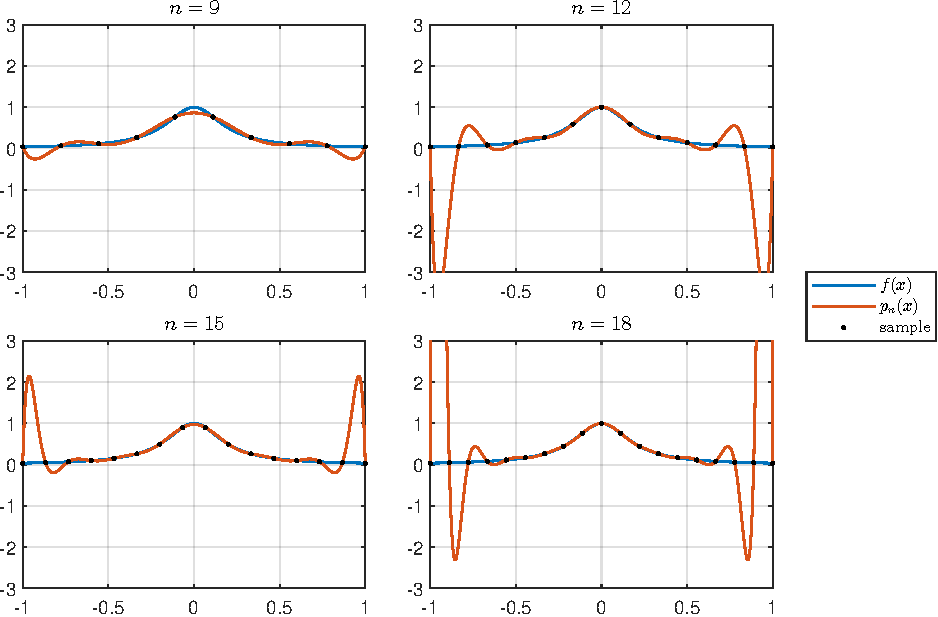
\includegraphics[width=0.8\linewidth]{graphs/Runge.pdf}
    \end{center}
    显然$f(x)$在$\RR$上是解析的,但在$\CC$上存在奇点$\pm\i/5$。
\end{example}

\section{分段插值}
\label{sec:piecewise interpolation}

\begin{definition}
    {分段线性插值}{}
    设
    \[
        a=x_0<x_1<\cdots<x_n=b,
    \]
    给定$f(x_i)$,找插值函数$\varphi$满足:
    \begin{itemize}
        \item $\varphi\in\cont[a,b];$
        \item $\varphi$在$[x_i,x_{i+1}]$上是线性函数。
        \item $\varphi(x_i)=f(x_i);$
    \end{itemize}
    满足前两个性质的函数组成插值空间$\Phi$,且$\dim(\Phi)=n+1$。
\end{definition}

\begin{theorem}
    {}{}
    插值函数是存在且唯一的。
\end{theorem}

\begin{proof}
    定义插值基函数
    \begin{equation}
        I_i(x)=\begin{cases}
            \frac{x-x_{i-1}}{x_i-x_{i-1}},&x\in[x_{i-1},x_i]\\
            \frac{x_{i+1}-x}{x_{i+1}-x_i},&x\in[x_i,x_{i+1}]\\
            0,&\otherwise
        \end{cases}
    \end{equation}
    则
    \begin{equation}
        \varphi(x)=\sum_{i=0}^nf(x_i)I_i(x).
        \qedhere
    \end{equation}
\end{proof}

\begin{theorem}
    {收敛性}{}
    定义$h:=\max_i(x_i-x_{i-1})$,
    \begin{itemize}
        \item 如果$f\in\cont[a,b]$,则$\lim_{h\to0}\norm{f-\varphi}_\infty=0;$
        \item 如果$f\in\cont^1[a,b]$,则$\norm{f-\varphi}_\infty\leq 2\norm{f'}_\infty h;$
        \item 如果$f\in\cont^2[a,b]$,则$\norm{f-\varphi}_\infty\leq \norm{f''}_\infty h^2/8;$
    \end{itemize}
\end{theorem}

\begin{definition}
    {分片三次Hermite插值}{}

\end{definition}

\section{Fourier插值}
\label{sec:Fourier interpolation}

\begin{definition}
    {Fourier级数}{}
    周期函数展开成Fourier级数
    \begin{equation}
        f(x)\sim\frac{a_0}2+\sum_{n=1}^\infty[a_n\cos(nx)+b_n\sin(nx)].
    \end{equation}
    其中
    \begin{subequations}
        \begin{align}
            a_n&=\frac1\pi\int_0^{2\pi}f(x)\cos(nx)\d x,\\
            b_n&=\frac1\pi\int_0^{2\pi}f(x)\sin(nx)\d x.
        \end{align}
    \end{subequations}
    \tcblower
    如果$f\in\cont^M$,则$a_n=\bigo(n^{-M}),\enspace b_n=\bigo(n^{-M})$,且
    \[
        \norm{f(x)-\fkh{\frac{a_0}2+\sum_{n=1}^N[a_n\cos(nx)+b_n\sin(nx)]}}_\infty=\bigo(N^{-M}).
    \] 
\end{definition}

\begin{definition}
    {三角多项式插值}{}
    给定周期为$2\pi$的函数$f$在节点$x_i=2\pi i/N$的值,希望重构函数$\psi$满足$\psi(x_i)=f(x_i)$。
    \tcblower
    寻找相多项式
    \begin{equation}
        p(x)=\beta_0+\beta_1\e{\i x}+\cdots+\beta_{N-1}\e{\i(N-1)x}.
    \end{equation}
\end{definition}

\begin{theorem}
    {}{}
    存在唯一的相多项式满足Lagrange插值条件且
    \begin{equation}
        \beta_j=\frac1N\sum_{k=1}^{N-1}f(x_k)\omega^{-kj},\quad\omega=\e{2\pi\i/N}.
    \end{equation}
    对应三角多项式为
    \begin{subequations}
        \begin{align}
            A_j&=\frac2N\sum_{k=0}^{N-1}f(x_k)\cos\biggkh{\frac{2\pi kj}N},\\
            B_j&=\frac2N\sum_{k=0}^{N-1}f(x_k)\sin\biggkh{\frac{2\pi kj}N},
        \end{align}
    \end{subequations}
\end{theorem}



